\documentclass[11pt,a4paper]{article}
\usepackage[hyperref]{emnlp2020}
\usepackage{times, graphicx}
\usepackage{latexsym}
\renewcommand{\UrlFont}{\ttfamily\small}
\usepackage{url}
\usepackage{microtype}
\usepackage{inconsolata}
\usepackage{booktabs}
\usepackage{hyperref}

\usepackage[utf8]{inputenc}
\usepackage[english]{babel}
\usepackage{ragged2e}
\usepackage{blindtext}
\usepackage{enumitem}
\usepackage{multirow}
\usepackage{subcaption}

\makeatletter
\newcommand{\printfnsymbol}[1]{
  \textsuperscript{\@fnsymbol{#1}}
}
\makeatother

\aclfinalcopy
\def\aclpaperid{0}

\setlength\titlebox{5cm}

\newcommand\BibTeX{B\textsc{ib}\TeX}


\newcommand\Warning{%
 \makebox[1.4em][c]{%
 \makebox[0pt][c]{\raisebox{.1em}{\small!}}%
 \makebox[0pt][c]{\Large$\bigtriangleup$}}}%
 
\newcommand{\noaug}{$\textrm{None}$}
\newcommand{\senttfpara}{$\textsc{SentenceParaphrase}$}
\newcommand{\tfpara}{$\textsc{Paraphrase}$}
\newcommand{\eda}{$\textsc{eda}$}
\newcommand{\synonym}{$\textsc{synonym}$}
\newcommand{\mlm}{$\textsc{mlm}$}
\newcommand{\mlmone}{$\textsc{mlm}_1$}
\newcommand{\mlmfive}{$\textsc{mlm}_5$}
\newcommand{\genaug}{$\texttt{GenAug}$}
\newcommand{\threshaug}{$\texttt{ThreshAug}$}
\newcommand{\vae}{$\textsc{vae}$}

\title{{\normalsize Social Computing Project: Final Report} \vspace{0.18cm} \\ Data Augmentation for Hate Speech Detection}

\author{Sayar Ghosh Roy\thanks{\ \ Equal contribution. Order determined by roll number.} \\ \texttt{20171047} \And
        Souvik Banerjee\footnotemark[1] \\ \texttt{20171094} \And
        Saujas Vaduguru\footnotemark[1] \\ \texttt{20171098} \And
        Ujwal Narayan\footnotemark[1] \\ \texttt{20171170}}

\date{}
\begin{document}
\maketitle

% \Warning This document contains samples of online social media hate speech which are present in the publicly available datasets we are currently studying. These are included for illustrative purposes only and in no way reflect the views of the authors. Please note that these samples are highly derogatory. Reader discretion is advised.

% \vspace{4mm}
% \hrule
% \vspace{4mm}

\section{Introduction}
As part of this course project, we explore different methods of improving hate speech detection models through data augmentation techniques. We consider the binary text classification formulation of the hate speech detection task. We select and formulate multiple diverse data augmentation techniques, and benchmark them against hate speech detection tasks based on datasets from multiple social media platforms including Reddit, Gab, and Twitter.

In this report, we describe the various augmentation approaches we have explored, our experimental pipeline, and our findings from the application of these approaches to the hate speech detection task. Our code (with all prior deliverables) are publicly available on GitHub at \url{https://github.com/sayarghoshroy/Augment4Gains}. Our presentation slides can be found \href{https://docs.google.com/presentation/d/1q8dZB-yR3A5ii-VkN5-RcjfE70lDnGSTHhFFtJ31EEM/edit?usp=sharing}{here}. Note that this report is a conspectus of our previous documents along with complete quantitative evaluation results. For more details on specific models, refer to our prior submissions.

\section{Data}
We focus on the data collected by \citet{benchmark}. Their dataset contains posts which are scraped from the Reddit\footnote{\url{www.reddit.com}} and Gab\footnote{\url{gab.com}} platforms, which typically have longer text samples, and tends to follow a more formal style than the posts on a platform like Twitter. The dataset contains human-annotated counter narratives specific to particular comment threads. In addition, they provide a list of indices of comments which contains instances of hate. We extract each user response in every post from these datasets separately and lookup the corresponding indices list to assign a binary label to every single user response, namely 1 for hateful, offensive or derogatory and 0 for otherwise. Each response, composed of multiple sentences is thus one datapoint.

As a pre-processing step, we remove information such as hashtags, mentions, URLs, emojis, etc. from every datapoint. We only leverage the cleaned text without any additional features for our augmented sample generation and classification tasks. For each dataset, we randomly divided the data in a 70:10:20 ratio (as done in \citet{benchmark}) into training, validation and testing splits (following the decision). Our processed Reddit dataset contains 15619 train samples, 2231 validation samples, and 4464 test samples while the processed Gab dataset carries 23643, 3377, and 6756 samples for training, validation, and testing respectively.

We also compare our methods with data from Twitter\footnote{\url{twitter.com}} \cite{gao-huang-2017-detecting}. Although our augmentation approaches are designed keeping a more formal style of English language text in mind, we will evaluate how each of these techniques work out on cleaned Tweet texts. Our processed Twitter dataset contains 17348 train samples, 2478 validation samples, and 4957 test samples. Throughout this document, we will refer to our three datasets as simply Reddit, Gab, and Twitter.

\section{Alteration-based methods}
\subsection{Non-contextual methods}
The first type of alteration-based methods we explore applies specific transformations to words in the input text without considering the sense in which these words are used.

\begin{figure*}
    \centering
    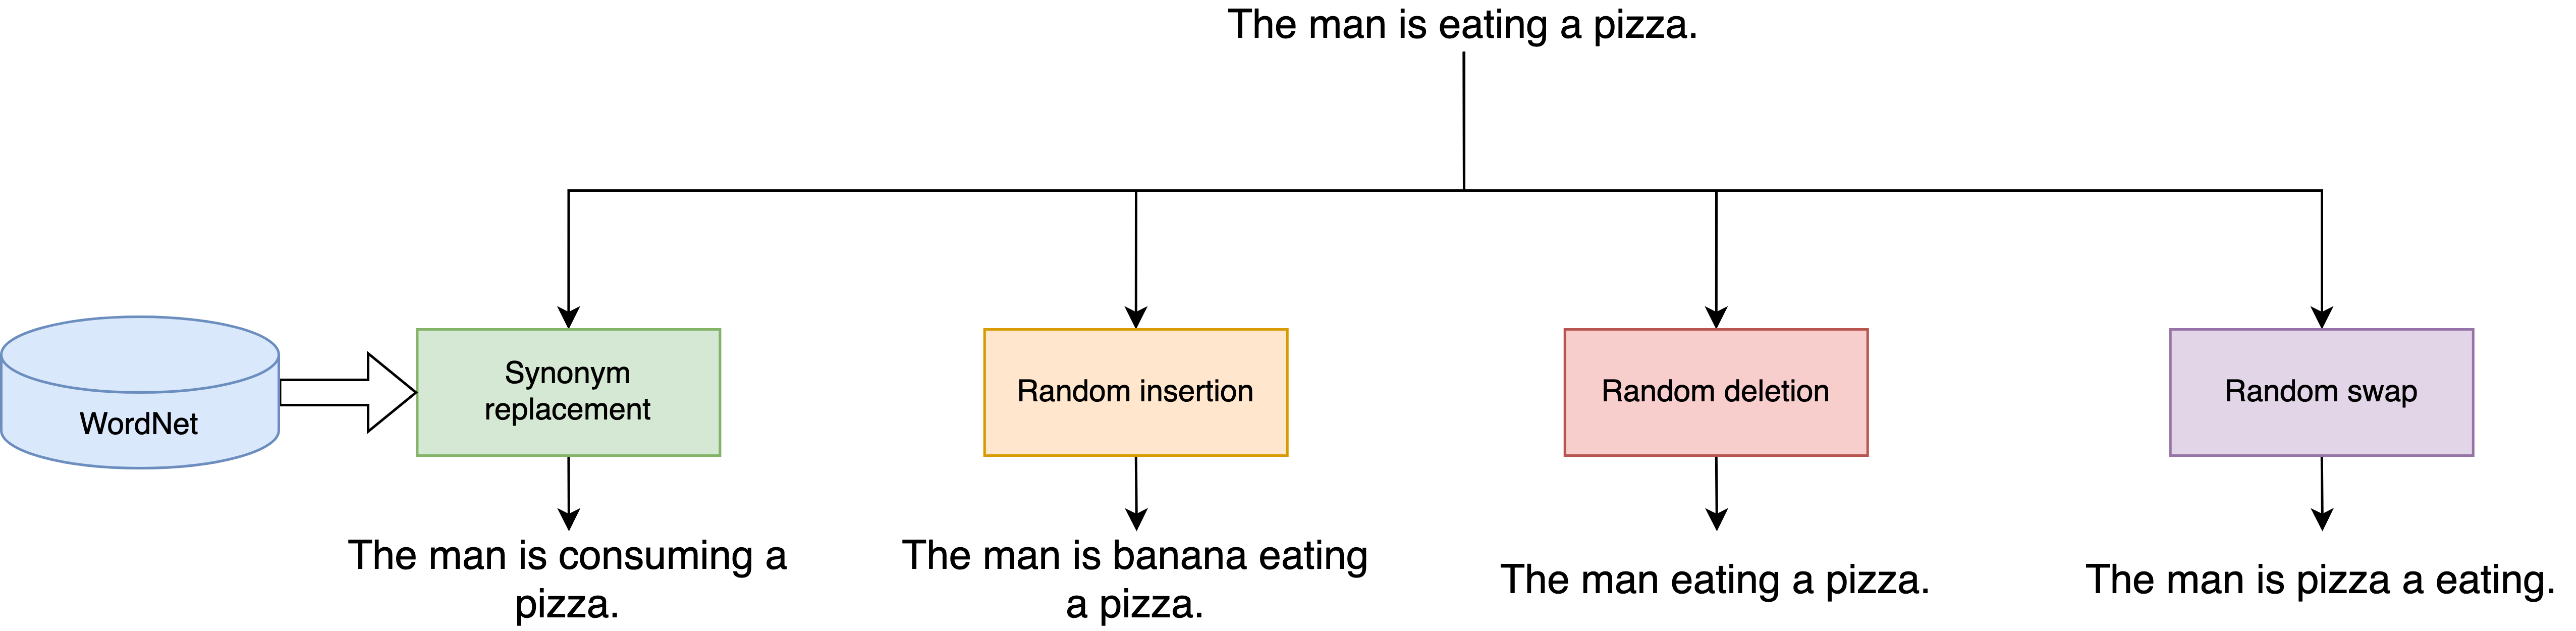
\includegraphics[width=\textwidth]{figs/eda.png}
    \caption{The easy data augmentation (EDA) pipeline.}
    \label{fig:eda}
\end{figure*}

\subsubsection{\texttt{ThreshAug}}
In order to make relevant substitutions of words with appropriate alternatives without access to a human-crafted knowledge base (such as a thesauraus, etc.), we make use of pretrained word embeddings (GLoVe in our actual implementation). This approach is adapted from the approach proposed by \citet{aug2prev}. These embeddings allow us to determine the relative similarity between each word in the vocabulary space of a text corpus. Now the question remains about which words to substitute. A substitution is determined by two factors. First, any potential replacement word must exceed the cosine distance threshold $t$, where $t \in  [0, 1]$ and it must match the POS-tag assigned to the word. The intuition behind the inclusion of both the above requirements is that two words must have been seen in sufficiently equal contexts such that one can be replaced with the other without changing the sentence semantics. We follow \citet{aug2prev} and use POS tags to choose words of only very specific tags like common nouns, adjectives and verbs. 

% This method, termed \textit{ThreshAug} forms a baseline for the alteration replacement approaches we explore.

\subsubsection{Easy Data Augmentation}

While there are a variety of techniques involved in data augmentation for text classification tasks, one of the most easiest yet surprisingly performant one is the Easy Data Augmentation (EDA) method \cite{wei-zou-2019-eda}. EDA consists of the following four basic operations. 

\begin{itemize}
\item \textbf{Synonym Replacement (SR)}: Here $n$ randomly selected words are replaced with one of it's synonyms chosen at random. These synonyms are generated by querying WordNet \cite{WordNet}, however it's important to note here that for synonym replacement all the senses of the word are considered and not just the sense in which it is currently being used. 
\item \textbf{Random Swap (RS)}: Here two words are randomly chosen from the sentence and their positions are swapped. This operation is repeated $n$ times
\item \textbf{Random Deletion (RD)}: Here each word of the sentence is randomly removed with the probability $p$.
\item \textbf{Random Insertion (RI)}: Here a randomly chosen synonym of a randomly selected word is inserted randomly into the sentence. This operation is then repeated $n$ times.
\end{itemize}

Figure~\ref{fig:eda} illustrates the pipeline with some hypothetical examples.

For operations such as SR, RI and RS, in order to prevent the new sentences from being too noisy we formulate $n$ to be dependent on the length of the sentence $l$, given by $n = \alpha l $ where $\alpha$ indicates the percentage of the sentence that will be modified. Other than these hyper-parameters, we also cap the number of generated sentences per source sentence with a parameter $n_{aug}$ so as to avoid pollution of the source data.

While the methods are simplistic and do not lead always lead to generation of high quality grammatically correct data, they have been shown to produce significant performance boosts.

% For the synonym specific operations, i.e. RI and SR only content words are chosen and the stop words are ignored. While the methods are simplistic and do not lead always lead to generation of high quality grammatically correct data, they produce significant performance boosts. \citet{wei-zou-2019-eda} also observe the newly generated sentences occupy positions closely around the original sentences in the latent semantic space and thus the meaning and therefore the labels do not significantly change. For operations such as SR, RI and RS, in order to prevent the new sentences from being too noisy we formulate $n$ to be dependent on the length of the sentence $l$, given by $n = \alpha l $ where $\alpha$ indicates the percentage of the sentence that will be modified. Other than these hyper-parameters, we also cap the number of generated sentences per source sentence with a parameter $n_{aug}$ so as to avoid pollution of the source data. 

\subsection{Contextual methods}
The second type of alteration-based methods we explore applies transformations to words in the input text based the sense in which these words are used.

\subsubsection{Synonym substitution}

\begin{figure}
    \centering
    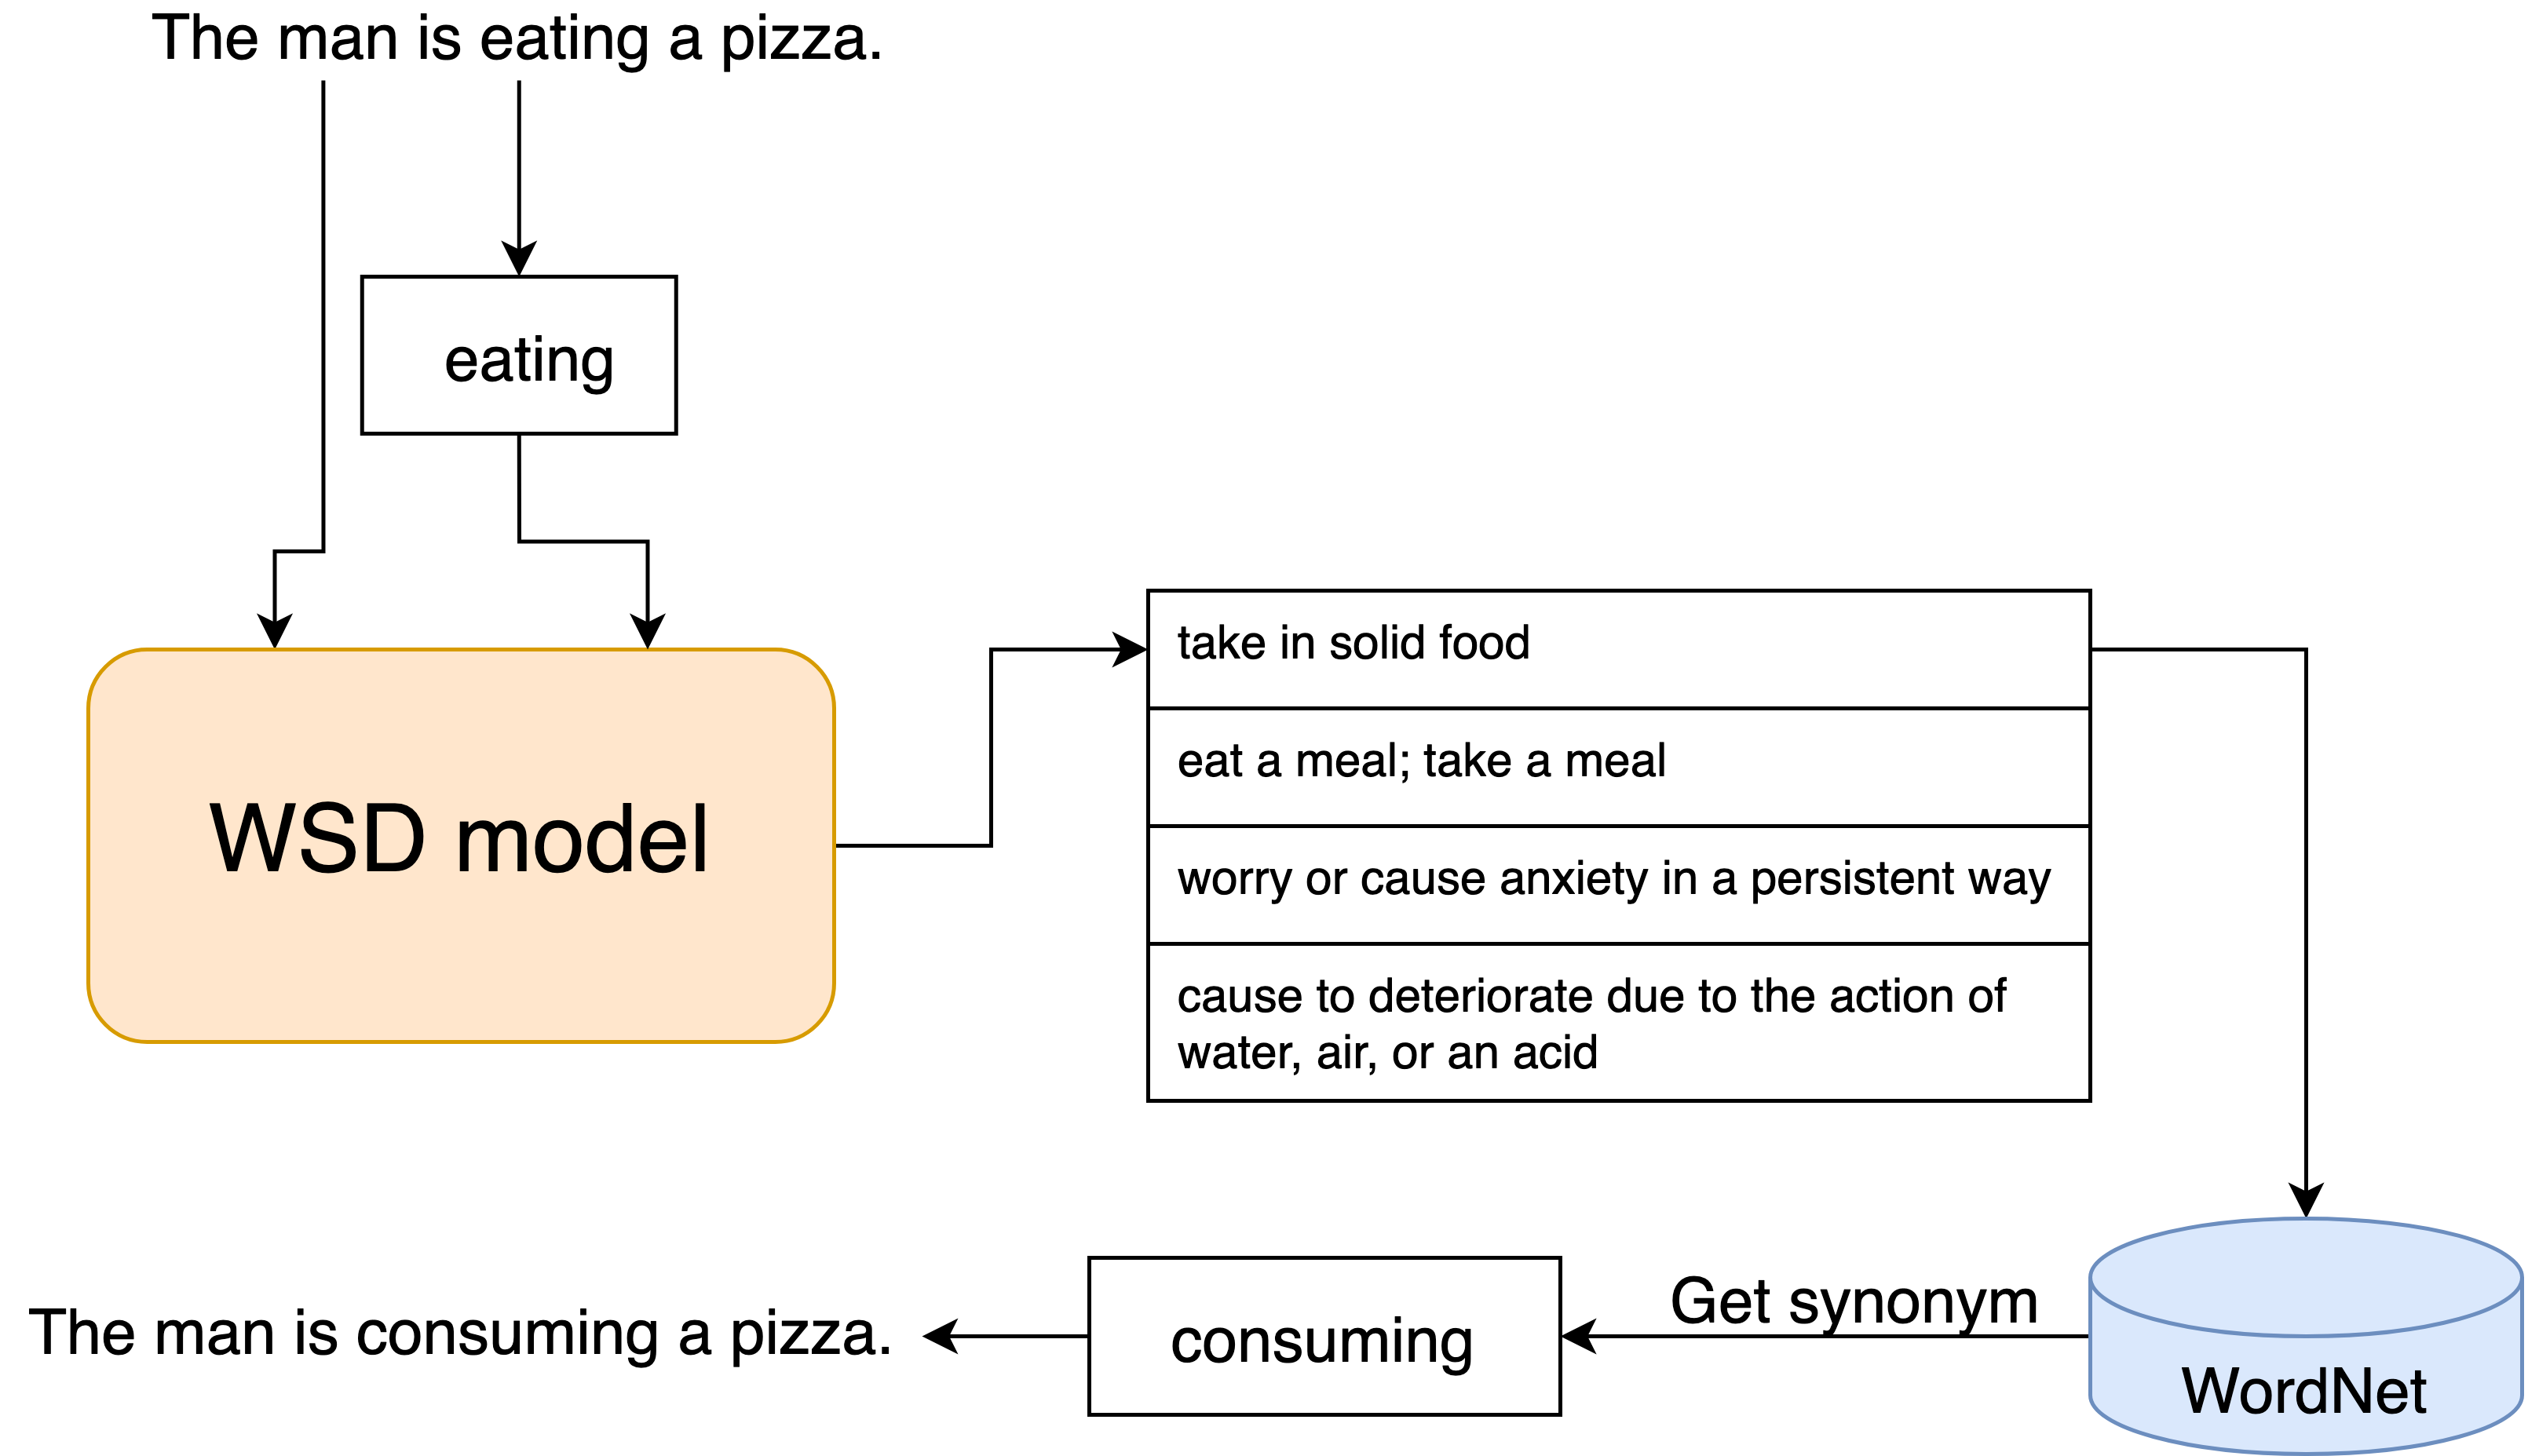
\includegraphics[width=\columnwidth]{figs/synonym.png}
    \caption{The \synonym\ pipeline.}
    \label{fig:wsd}
\end{figure}

When augmenting samples by substituting words with their synonyms. it becomes important to identify the right sense of the word so that the right synonyms of that word can be found. We follow  the approach  of \citet{yap-etal-2020-adapting} to perform \textit{word sense disambiguation} and identify the WordNet sense to which the word that is used corresponds.

To perform WSD, we first need to identify the right phrases to substitute or replace and thus we chunk the sentence. Once the sentence is split into multiple chunks, we check if that particular chunk is present in WordNet. If it is present, we then leverage BERT to rank all the senses of the word in the context of the sentence. We pick the sense with the highest rank as the correct sense of the word. If the chunk is not present in WordNet , we back-off and search through all the words of the chunks individually and repeat the process we mentioned earlier to identify the sense of the word. Once we found the right sense of the word, we query WordNet again to retrieve the set of synonyms and hypernyms associated with the particular word or phrase. Once we have the synonyms, we substitute these synonyms in-place of the original word or phrase to generate new samples for training. 

This method leverages both BERT and WordNet \cite{WordNet} to find the right sense of the word. We term this augmentation method \synonym, and illustrate the pipeline in Figure~\ref{fig:wsd}.

\subsubsection{Masked language modelling-based substitution}

\begin{figure}
    \centering
    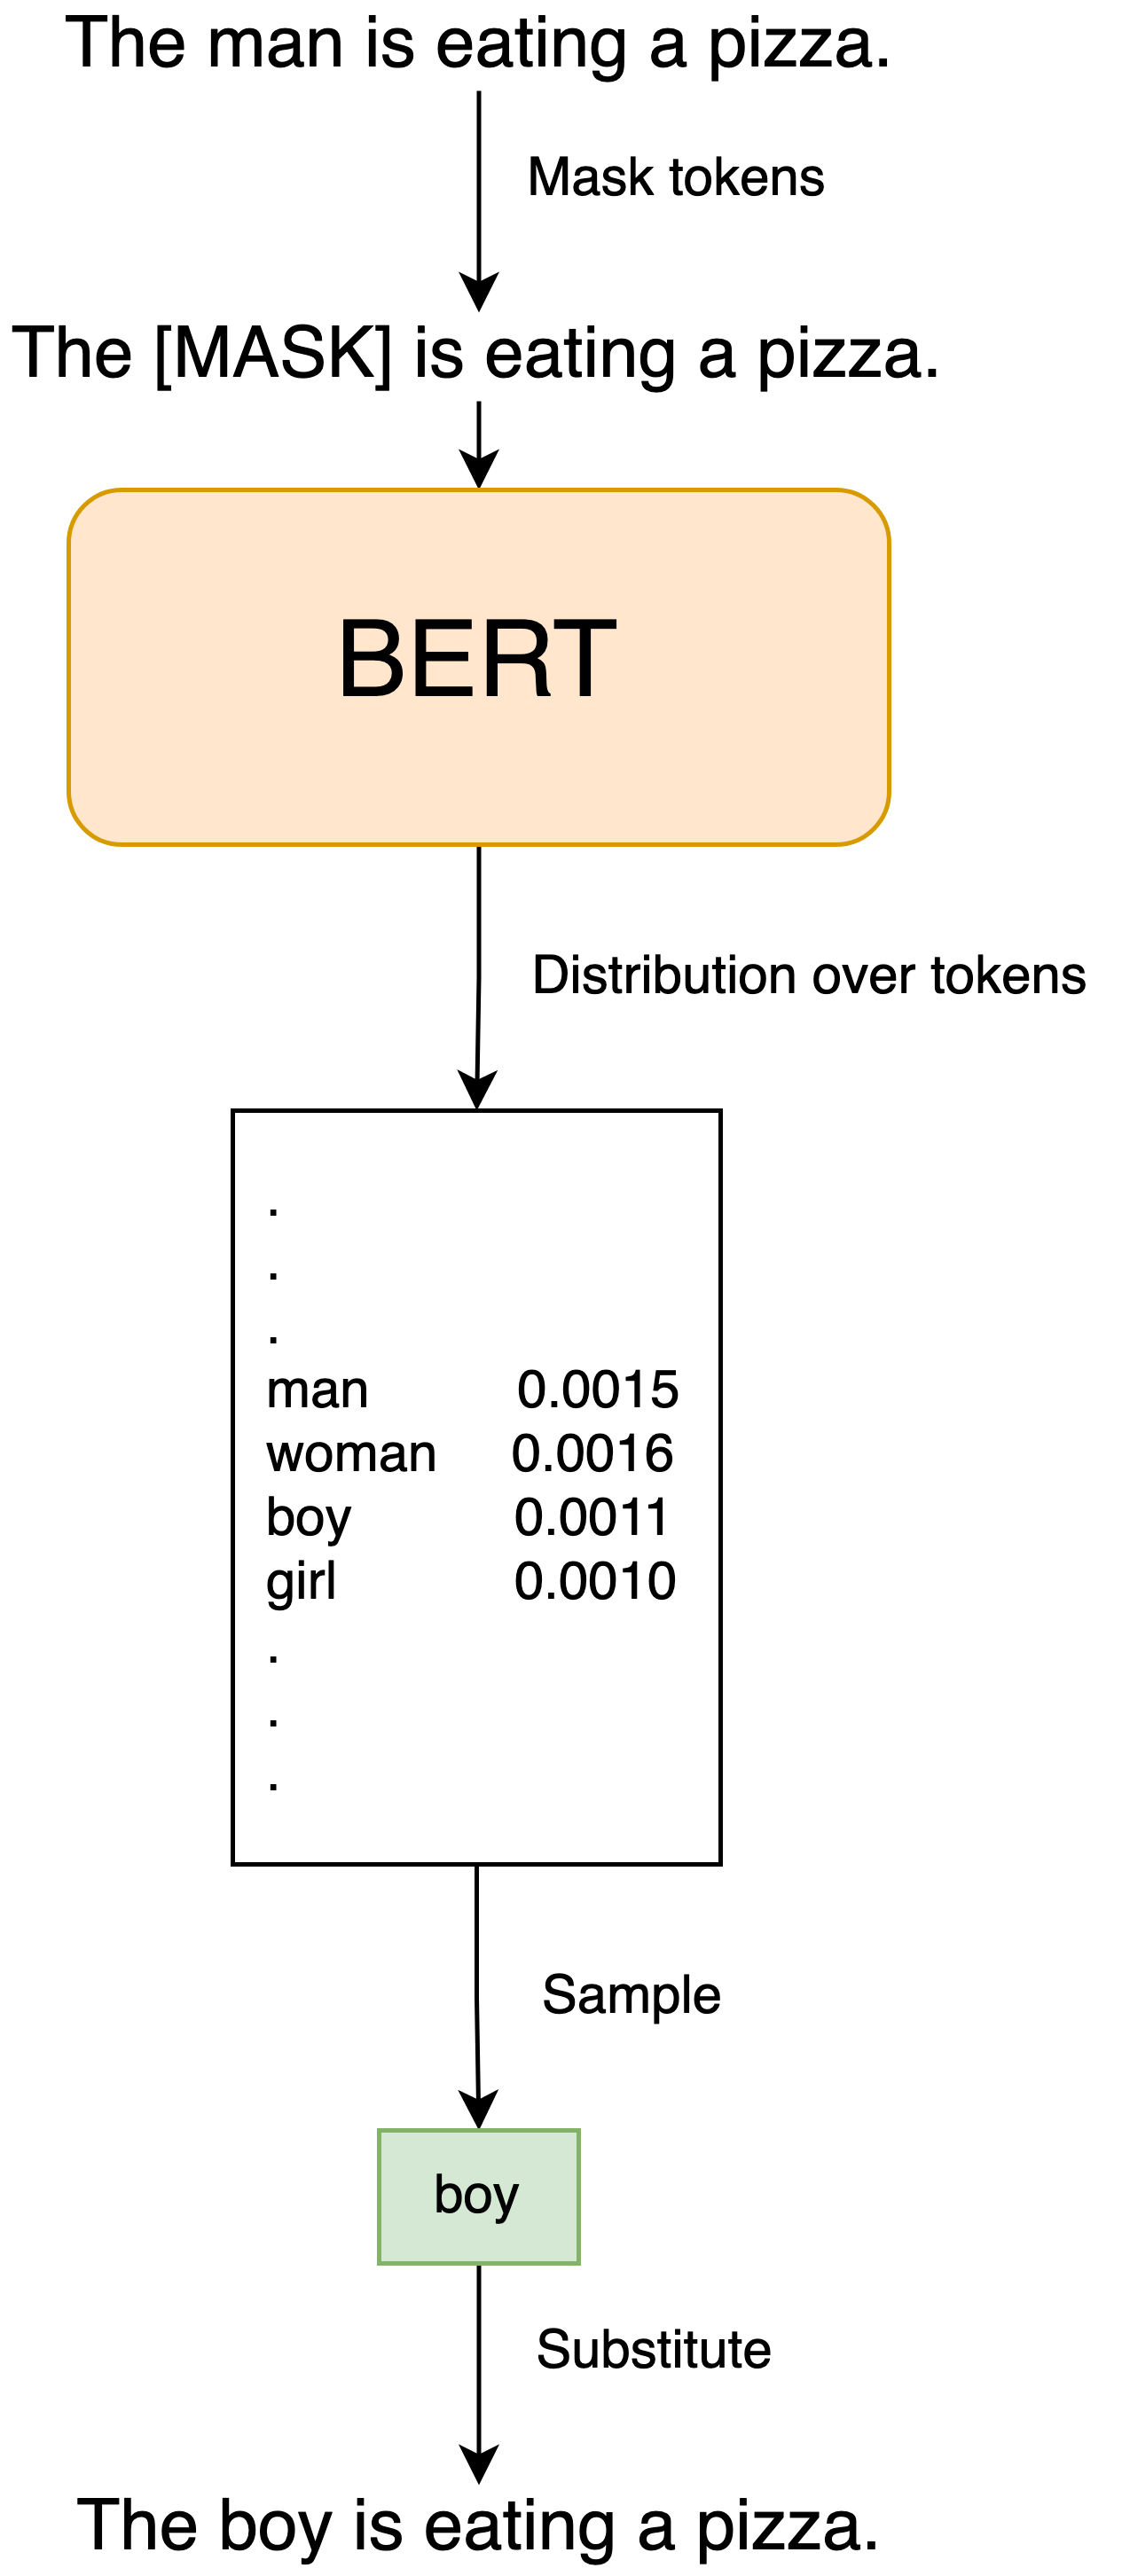
\includegraphics[height=10cm]{figs/mlm.png}
    \caption{The \textsc{mlm} pipeline.}
    \label{fig:mlm}
\end{figure}

With the advent of contextualized word representations \cite{peters-etal-2018-deep,devlin2018bert}, we have access to methods that can compute word embeddings that can allow for sense disambiguation based on context. \citet{kobayashi-2018-contextual} propose using contextual embeddings in the data augmentation pipeline for text classification tasks. Similar to \citet{aug2prev}, who select words for substitution and determine the alternatives using word embedding similarity, \citet{kobayashi-2018-contextual} select words to substitute, and use a bidirectional language model to choose the word to be substituted. 

Using the language model, they obtain the distribution $p(w_i'|S \setminus \{w_i\})$, where $S$ is the sample, $w_i$ is the word chosen for substitution, and $w_i'$ is the alternative word. Then, they sample from the distribution $p(w_i'|S \setminus \{w_i\})$, which is the distribution predicted by the model.

We use a pretrained BERT model with an MLM head to generate samples for augmentation. We choose whole words (as opposed to tokens in the TLM vocabulary, which tend to be subwords) with a fixed probability, and replace these words in the data with the \texttt{[MASK]} token. We then pass these to a TLM with the MLM head, and obtain the distribution over tokens that can fill the \texttt{[MASK]} token. This distribution, which is equivalent to $p(w_i'|S \setminus \{w_i\})$, is then used to sample replacements and obtain augmented samples. This pipeline is illustrated in Figure~\ref{fig:mlm}. We use this technique to augment data to two different degrees -- one sample for each training sample (\mlmone) and five samples for each training sample (\mlmfive).

\section{Generation-based methods}
In addition to methods that generate new samples by applying transformations to words in input text, we also explore methods where an augmentation sample is generated from scratch, constrained either by the class of the generated sample, or by the meaning of a training sample.

\subsection{Class-based generation}
We present two methods to generate samples constrained only by the class label. The first is a baseline method proposed by \citet{aug2prev} called \texttt{GenAug}. The second is an approach based on Variational Autoencoders (VAEs).

\subsubsection{\texttt{GenAug}}
The main idea behind GenAug is extremely similar to that of using RNNs (LSTMs/GRUs) for Natural Language Generation. Training such a model is synonymous to training a word level language model. Hence, for making inferences using such models, we start with a random word from the vocabulary and attempt to predict each in-sequence next word based on the generation so far. Our implementation, specifically takes N words as input and converts each into a 100-dimensional word embedding vector. This sequence of vectors is then passed through a bidrectional-LSTM layer with 128 hidden units each. Finally, the output of the bi-LSTM is fed into a final FCNN layer. The final output represents a probability distribution over each token in the vocabulary the argmax of which produces the output token. We train one model for each class, and use it to generate 2000 samples (1000 for each label) for augmentation (except in the data balanced setting).

\subsubsection{Variational autoencoder}

\begin{figure*}
    \centering
    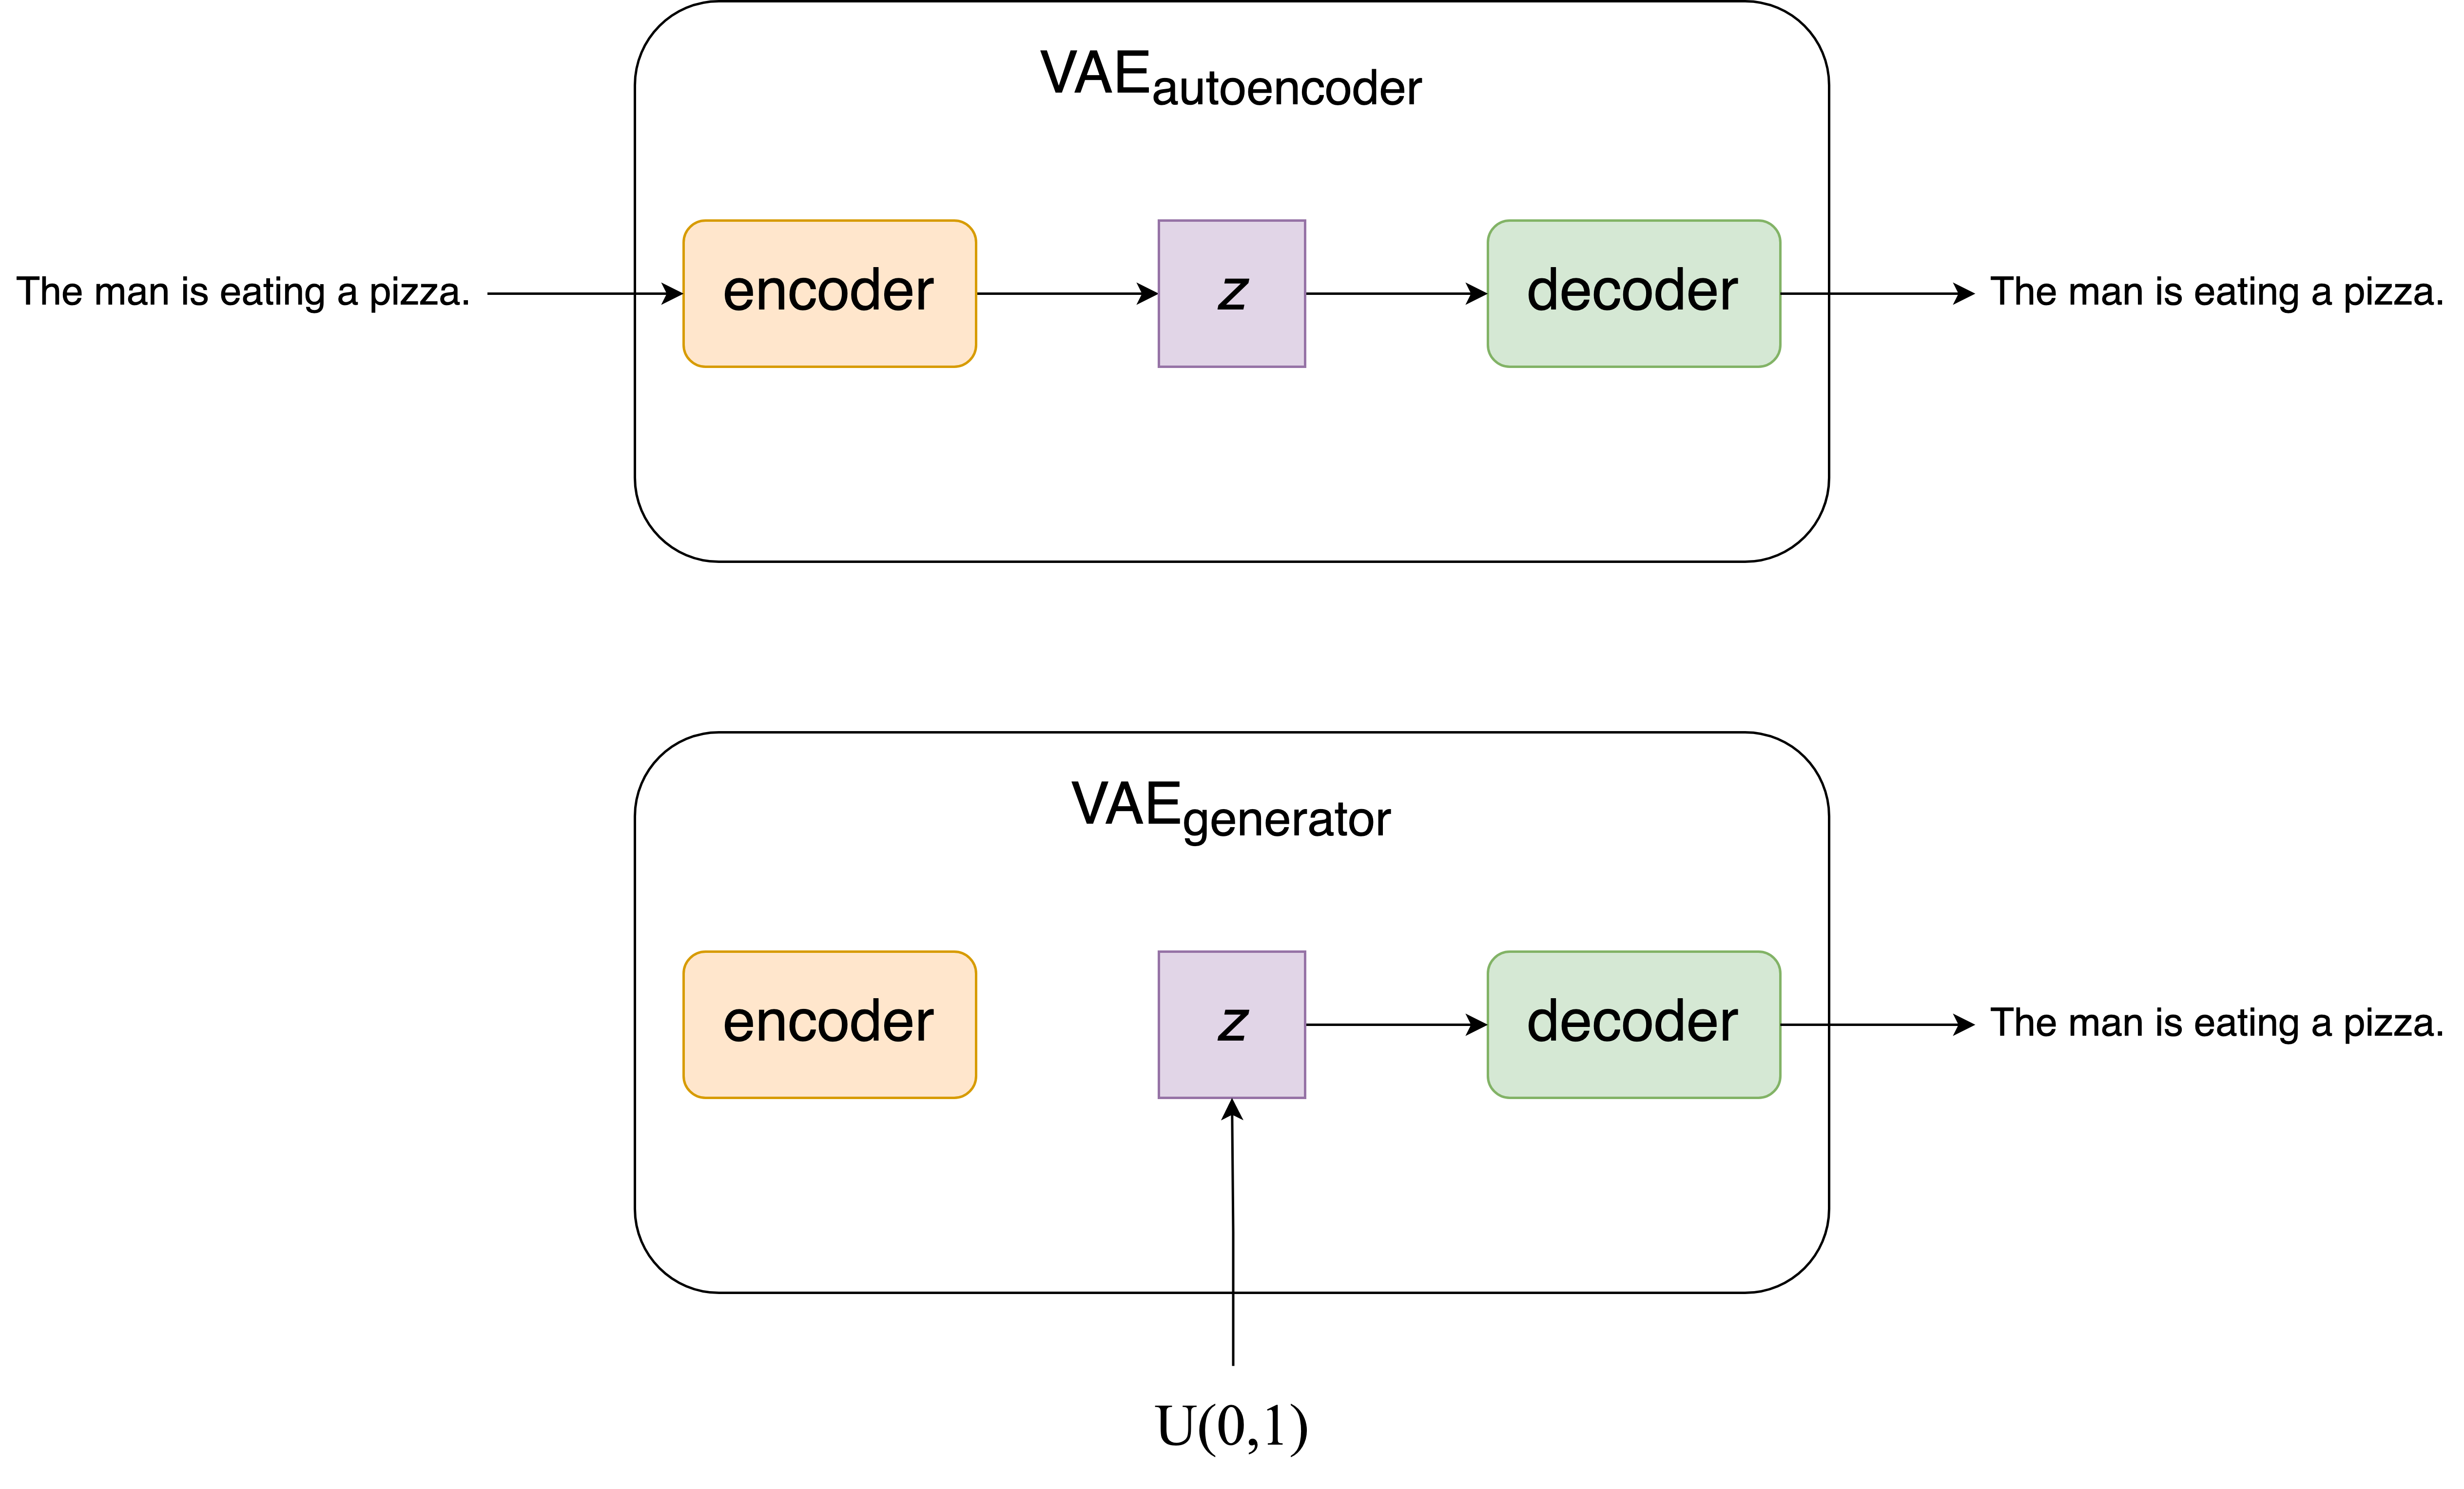
\includegraphics[width=\textwidth]{figs/vae.png}
    \caption{The \textsc{vae} pipeline.}
    \label{fig:vae}
\end{figure*}

We also explore the use of VAEs for generating samples within each class. We adopt the approach presented by \citet{bowman-etal-2016-generating}. The model is trained as an autoencoder with an encoder function $f_{enc}(x)$ that maps an input $x$ to a learned code $z$, and a decoder function $f_{dec}$ that recovers $x$ from the code $z$. The model is trained to recover the input (with the difference forming one loss term) while keeping the posterior distribution $q(z|x)$ modelled by $f_{enc}$ close to a prior $p$ (with the Kullback-Leibler divergence between $p$ and $q$ forming the second loss term). For the application of text representation learning, the functions $f_{enc}$ and $f_{dec}$ are parametrised as recurrent neural networks.

We train a single VAE model for each class, and then generate samples for each class by sampling a random point $z' \sim \mathcal{U}(0, 1)$ in the latent space of the model's learned code, and using the decoder to generate a sequence conditioned on $z'$. The intuition here is that a model corresponding to a particular class learns a latent space of codes corresponding to the distribution of samples in that particular class. Then, any point in that latent space is the representation of some sample belonging to that class, and we can decode that sample by conditioning on the point in the latent space.

We adapt an implementation of \citet{bowman-etal-2016-generating}\footnote{\url{https://github.com/timbmg/Sentence-VAE}} for our application. The pipeline for \vae\ is illustrated in Figure~\ref{fig:vae}. We generate one sample of the same class for each sample in the training data.

\subsection{Paraphrasing methods}
Paraphrases can be defined as sentences conveying the same meaning but with different surface realizations. In this report, we use ``augmentation through paraphrasing" to only refer to the paraphrases generated from scratch as paraphrases generated through substitutions or replacements have been covered earlier under alteration-based methods.

We utilize a fully trained Transformer-based sequence to sequence architecture for paraphrase generation. Instead of randomly initializing the Transformer weights prior to fine-tuning, we choose a pretrained Transformer model that has already `witnessed' and learnt from large chunks of natural language text. Such a pretrained text-to-text Transformer is then fine-tuned auto-regressively on supervised input-source to paraphrased-target mappings.

After manually studying the qualities of various output sentences from these pretrained Transformer encoder-decoder models, we found that PEGASUS produces the best looking sequences with the least amount of noticeable grammatical errors (something which is corroborated in their publication as well). Therefore, we chose to utilize PEGASUS as our base pretrained Transformer model for the paraphrasing task. We used Hugging Face's implementation of PEGASUS\footnote{\url{huggingface.co/transformers/model_doc/pegasus.html}} with number of beams for decoding set to 10, a maximum sequence length of 128, with all other hyperparameters set to their default values.

For training an encoder-decoder model for paraphrasing, only the true-labelled sentence pairs from the \texttt{PAWS-Wiki} and \texttt{PAWS-QQP} datasets are considered. These can be regarded as the gold standard for the paraphrase recognition task since all of their supervised samples are based on human judgements. \texttt{PAWS-Wiki} \cite{paws} contains a collection of sentence pairs sourced from Wikipedia labelled for whether one sentence is a paraphrase of the other. Similarly, \texttt{PAWS-QQP} contains contains pairs of Quora questions with similar paraphrase-worthiness labels.

We experiment with two modes of inference with paraphrasing models:
\begin{itemize}
    \item \tfpara: Pass the entire training sample to the paraphrasing model as input. We found that the outputs tend to focus on the initial part of the input, and lose information in the later parts of the input.
    
    \item \senttfpara: To address the information loss, we generate paraphrases for each sentence in the input sample independently and concatenated sentence-specific paraphrases to produce a comprehensive paraphrase for the complete sample.
\end{itemize}

We also explored the use of VAEs used as autoencoders for paraphrasing, but did not pursue the line of investigation as inspections of the generated samples revealed that the generated paraphrases were of poor quality.

\section{Experiments}
\subsection{Classification model}
Fine-tuning of pretrained Transformer models such as BERT \cite{devlin2018bert} and RoBERTa \cite{roberta} is becoming the new baseline for various tasks in the NLP domain. For evaluating our data augmentation approaches, we utilize a pretrained models (BERT and RoBERTa) as text encoders, paired with a Multi-Layer Perceptron (MLP) classifier head that considers the final-layer output embedding of the \texttt{[CLS]} token. We utilize the Adam optimizer to train our classification architecture for a total of 4 epochs and save the model weights corresponding to the point in training that manifested the least validation loss.

\subsection{Test Bench}
We require a uniform scheme of evaluating all of our augmentation approaches. Therefore, for each dataset under consideration (be it Reddit, Gab, or Twitter), we lock the validation and the testing data. All the augmented examples are based solely on the training samples. This is to ensure that there is no seepage of information and as such, the classification models do not indirectly look at some modified version of a test (or validation) sample.

Every augmentation method can be viewed as an algorithm that takes in a sample of text as input conditioned on which one or more revamped samples are produced. In our pipeline, the in-question augmentation procedure is applied to all the training datapoints. The generated samples are appended to the existing training split resulting in the augmented train data-frame. The classification test-bench utilizes the newly created training set, taking care of the downstream steps. Figure~\ref{fig:pipeline} illustrates the complete experimental pipeline we adopt.

\begin{figure}
    \centering
    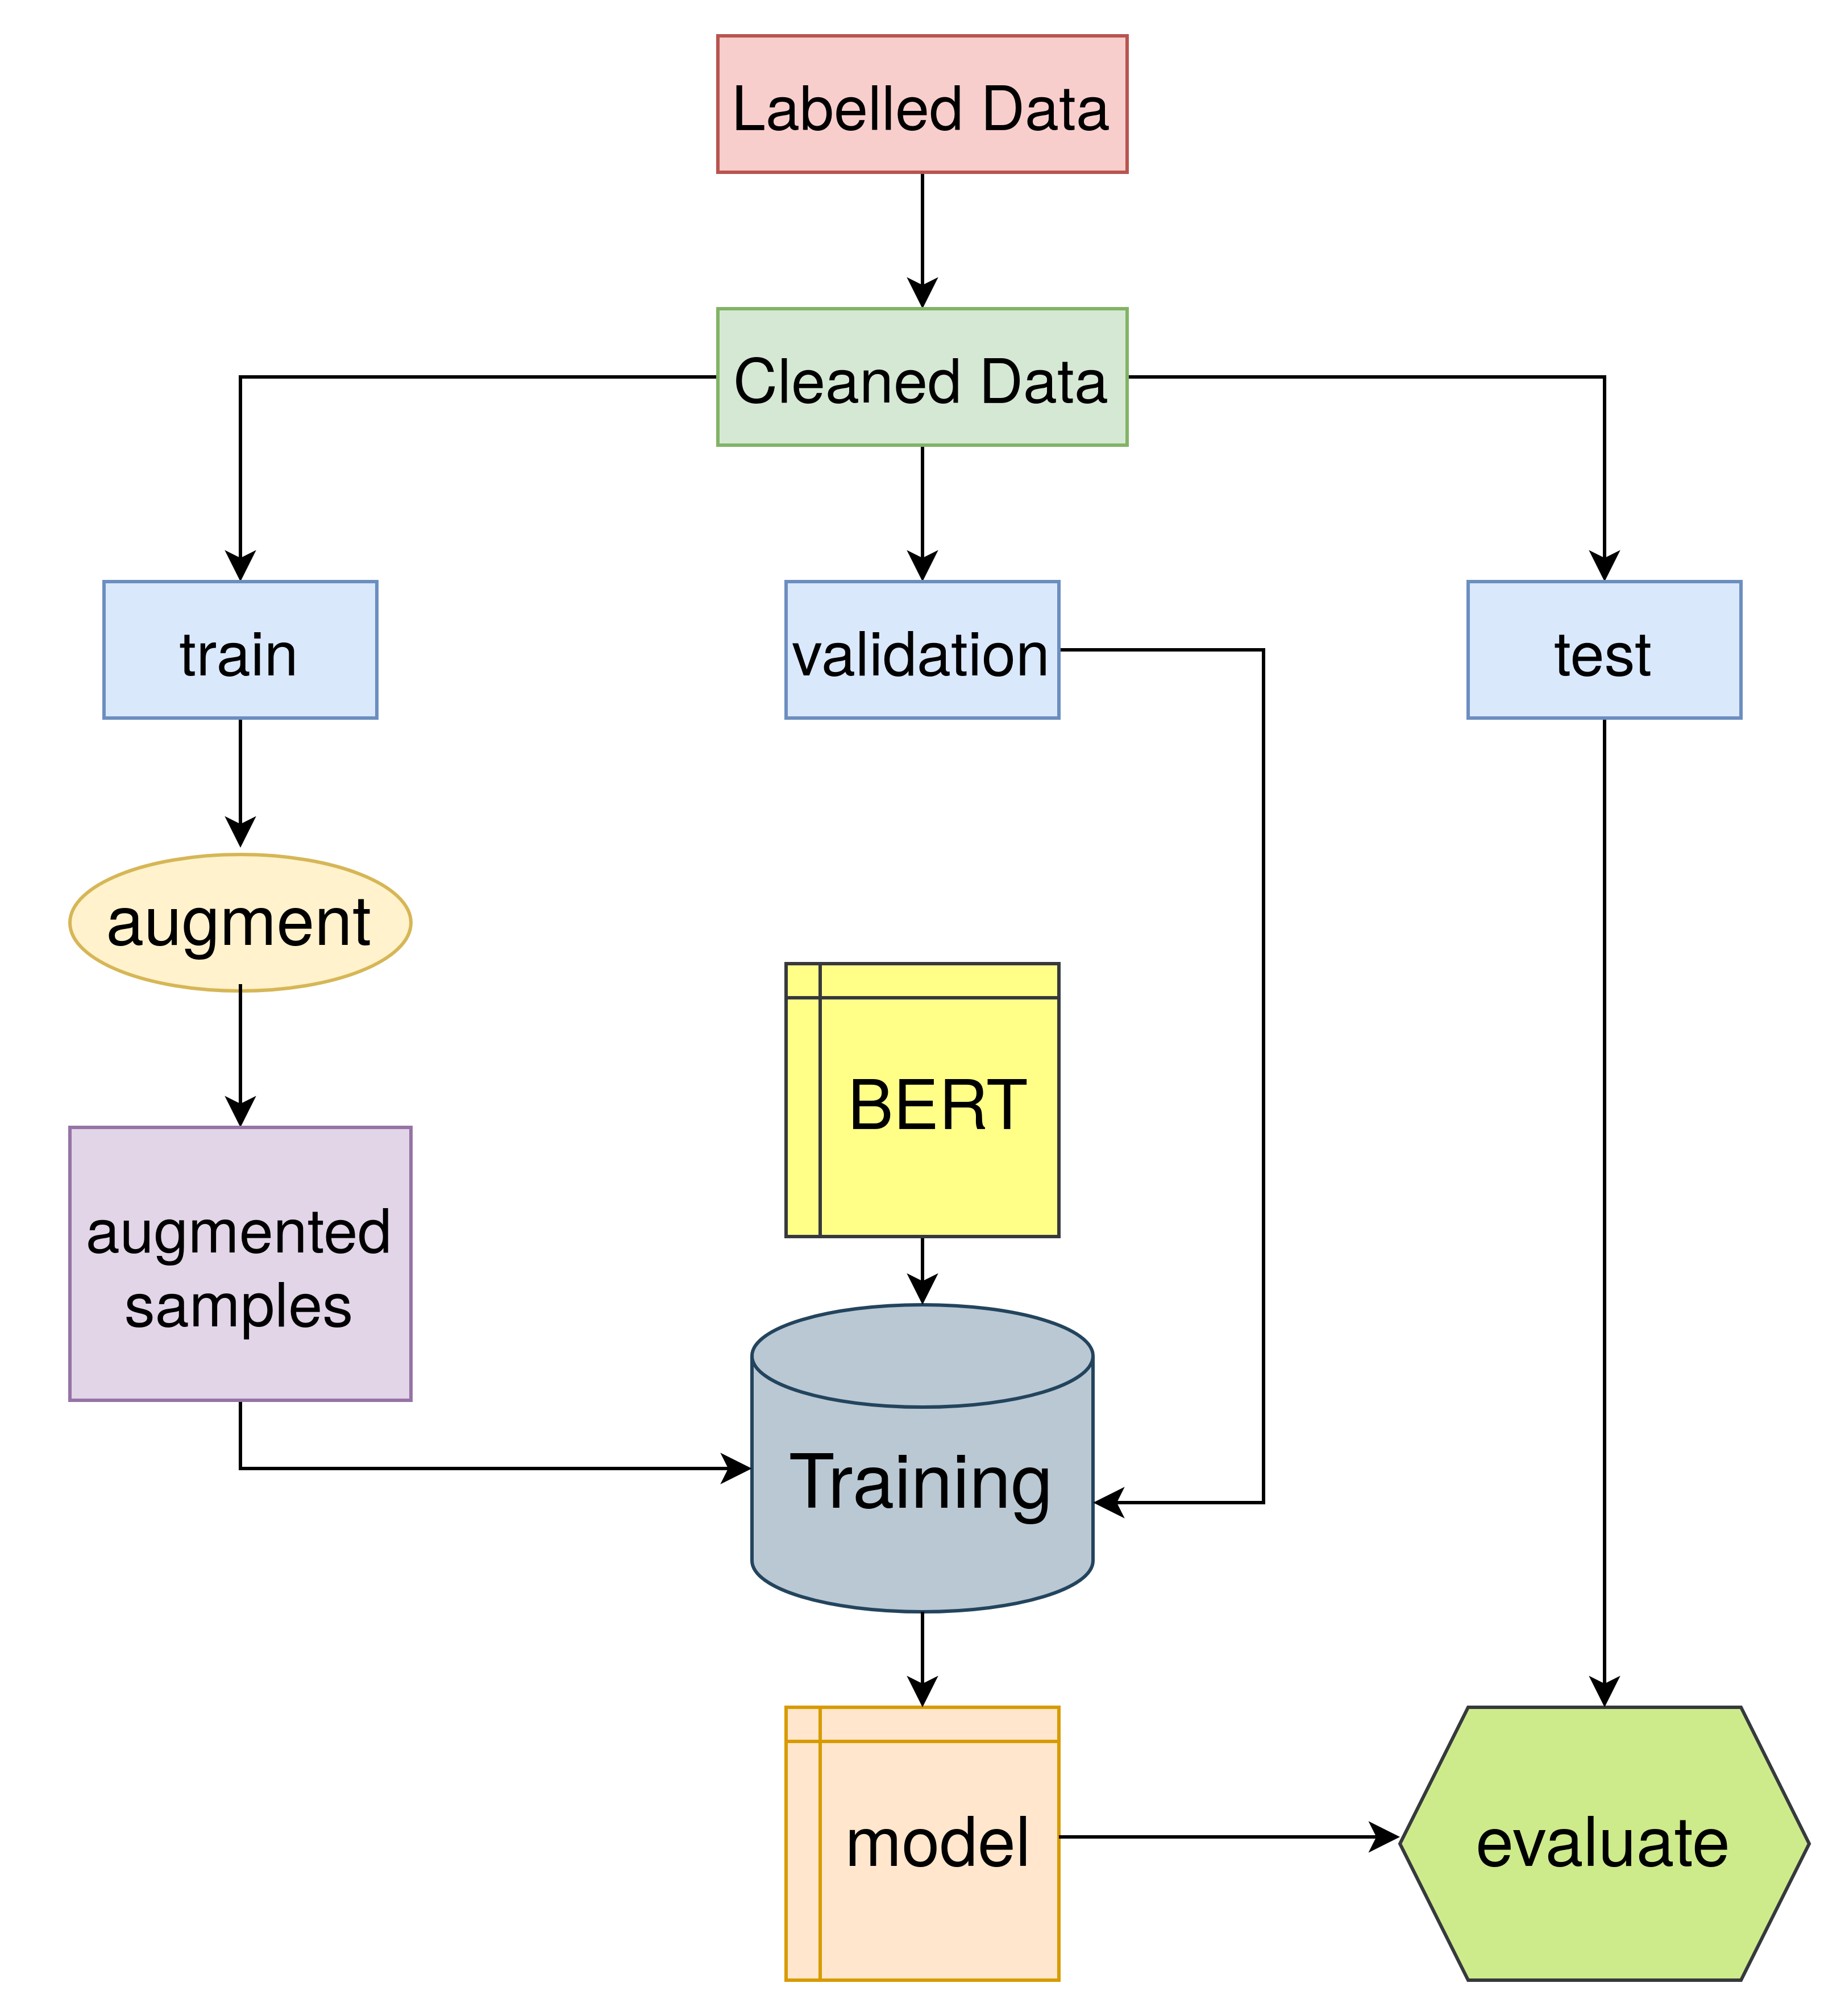
\includegraphics[width=\columnwidth]{figs/pipeline.png}
    \caption{Our complete experimental pipeline}
    \label{fig:pipeline}
\end{figure}

\subsection{Class balancing}
To address the class imbalance in the datasets we consider two approaches.

\subsubsection{Class balancing in the loss function}
One way of dealing with class imbalance in the base as well as some of the augmented datasets is to weigh each class differently in the loss function during training.

We implement the option of weighing terms in the classifier loss accordingly to counter the effects of class imbalance. We use two different ways of weighing the terms in the loss function:
\begin{itemize}
    \item Type-1: 
    \begin{itemize}
        \item Weight for positive sample: $\frac{\max \{N, P\}}{P}$
        \item Weight for negative sample: $\frac{\max \{N, P\}}{N}$
    \end{itemize}
    \item Type-2:
    \begin{itemize}
        \item Weight for positive sample: $\frac{N + P}{2P}$
        \item Weight for negative sample: $\frac{N + P}{2N}$
    \end{itemize}
\end{itemize}

where $P$ is the number of positive samples, and $N$ is the number of negative samples.

\subsubsection{Class balancing by augmentation}
Another way is to differentially augment the classes to reduce the class imbalance. Here, we augment samples to equalize the numbers of samples in the classes. Using the techniques presented before, we generate sufficient quantities of augmentation samples for each class. Then we augment each class with enough samples to make the total number of samples in the augmented training data for each class equal to 15000. This addresses the class imbalance problem by augmenting samples to amend this imbalance. We term this method as data balancing.%balancing by augmentation.

\begin{table*}[]
    \small
    \centering
    \begin{tabular}{cllcllc}
    \toprule
        \multirow{2}{*}{\textbf{Dataset}} & \multicolumn{3}{c}{\textbf{BERT}} & \multicolumn{3}{c}{\textbf{RoBERTa}} \\\cmidrule(lr){2-4}\cmidrule(lr){5-7}
         & \textbf{Augmentation} & \textbf{Balancing} & \textbf{Accuracy} & \textbf{Augmentation} & \textbf{Balancing} & \textbf{Accuracy} \\
         \midrule
         Reddit & \senttfpara & None & 92.3611* & \tfpara & None & 92.2267*\\
         Gab & \senttfpara & Type-2 & 92.6732 & \senttfpara & None & 92.7916 \\
         Twitter & \mlm & Data & 96.1267 & \threshaug & None & 95.9855* \\
    \bottomrule
    \end{tabular}
    \caption{Most accurate models}
    \label{tab:bestmodels}
\end{table*}

\section{Results}

Table~\ref{tab:bestmodels} shows the performance of the best (most accurate) augmentation methods on each dataset\footnote{* indicates that a model without augmentation outperforms this model under some class balancing method.}. Our full results, grouped by dataset, and further by class balancing method, are presented in Appendix~\ref{sec:fullresults}. 

We find that the effectiveness of augmentations varies across datasets as well as choice of pretrained encoder models. While \senttfpara\ is found to work well with BERT, other augmentation methods are seen to perform well with RoBERTa. We also see that different augmentation methods, combined with different methods of class balancing perform best on each dataset. In some cases, the class balancing alone provides the best performance.

\subsection{Comparison of augmentation paradigms}
An interesting phenomenon we observe is that on Reddit and Gab data, we find generation-based augmentation methods doing well, while on Twitter data, the best performing augmentation methods are both alteration-based methods. One possible reason for this could be the stylistic differences between Twitter data and Reddit and Gab data that motivated our focus on Reddit and Gab in the first place.

On Reddit and Gab data, we find that Transformer-based paraphrasing methods perform well. This augmentation method provides improvements with both BERT and RoBERTa models, and is the best performing augmentation method on data that typically has longer form, slightly more formal style of text. Another encouraging and interesting finding is that these paraphrasing models are robust to a move away from their training domain (Wiki and Quora), and are able to provide improvements even on Reddit and Gab data. This suggests the direction of exploring Transformer-based paraphrasing as an augmentation method in other domains and tasks as well, to harness the ability of these models to capture patterns in language in a powerful and robust way.

In contrast, we find that alteration-based augmentation methods, which have been shown to provide improvements in other settings, do not perform well in this setting. In most cases, on Reddit and Gab data, alteration-based augmentation leads to degradation of performance. 

\subsection{Comparison of class balancing methods}

\begin{figure*}
    \centering
    \begin{subfigure}{1.5\columnwidth}
        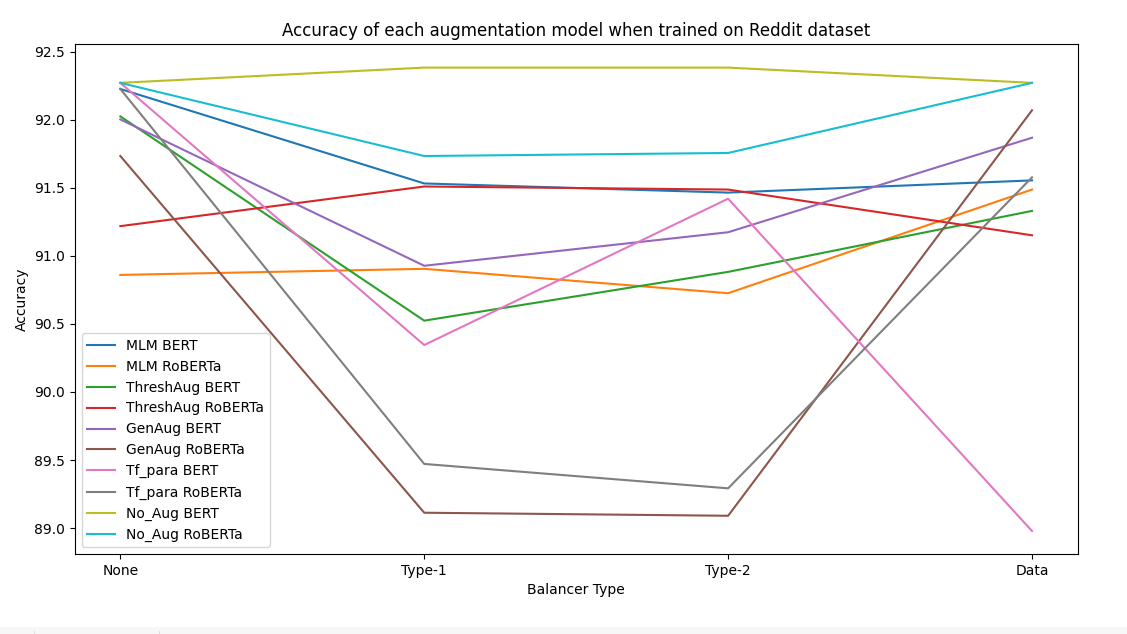
\includegraphics[width=\columnwidth]{figs/reddit.png}
        \caption{Reddit}
        \label{fig:redditbal}
    \end{subfigure}
    
    \begin{subfigure}{1.5\columnwidth}
        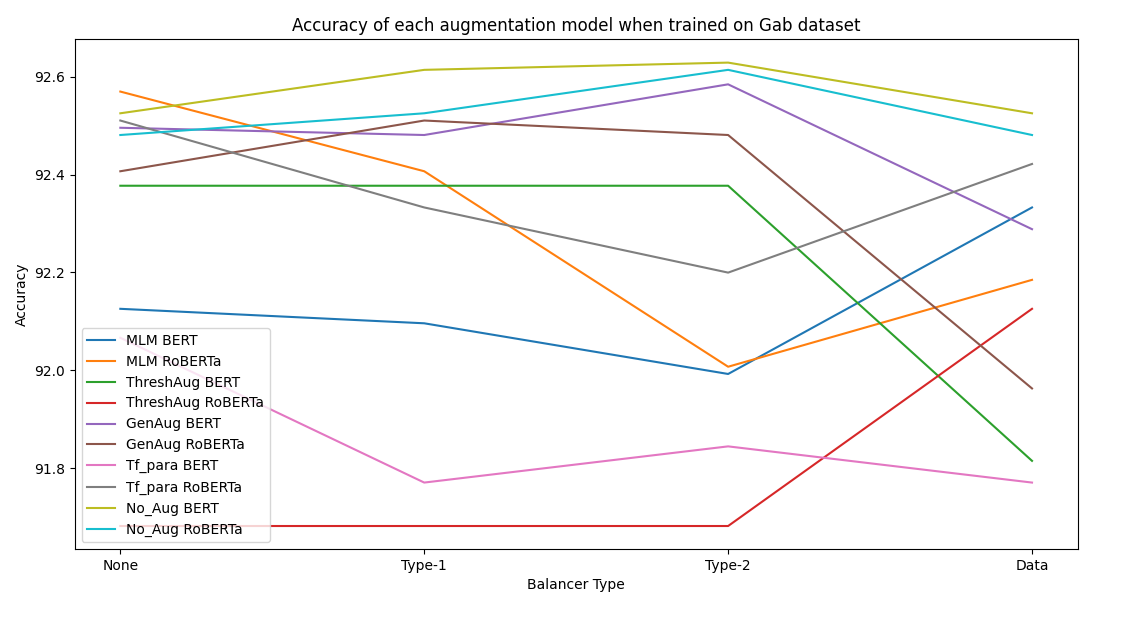
\includegraphics[width=\columnwidth]{figs/gab.png}
        \caption{Gab}
        \label{fig:gabbal}
    \end{subfigure}
    
    \begin{subfigure}{1.5\columnwidth}
        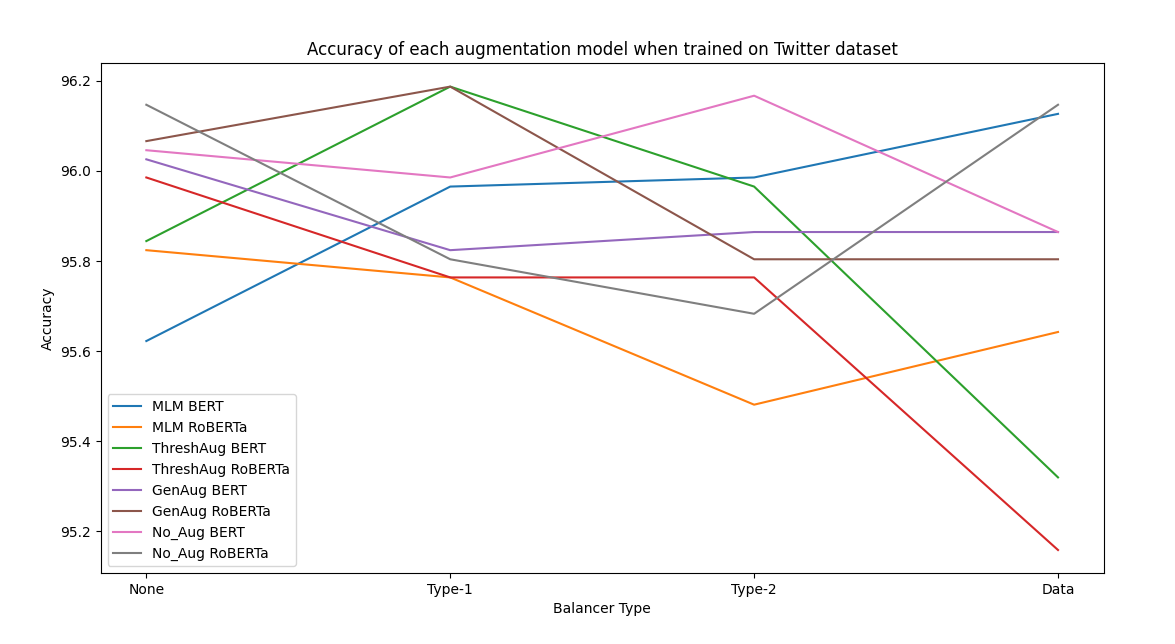
\includegraphics[width=\columnwidth]{figs/Twitter.png}
        \caption{Twitter}
        \label{fig:twitterbal}
    \end{subfigure}
    \caption{Accuracy of different models when combined with different class balancing methods (no balancing, type-1, type-2, and data balancing repsectively).}
    \label{fig:bal}
\end{figure*}

Figure~\ref{fig:bal} shows how the accuracy of a the classification model varies based on the class balancing method. We find that for Reddit data, type-1 and type-2 balancing work well when no augmentation is performed, but tends to degrade performance when used in conjunction with augmentation methods. Data balancing on the other hand works best among the class balancing methods on Reddit. We see a similar trend for Gab data in some cases, although in others type-2 balancing outperforms data balancing, reversing the trend. 

However, examining similar results on Twitter data does not reveal such a clear trend, further highlighting the qualitative differences between Reddit or Gab, and Twitter data.

\bibliographystyle{acl_natbib}
\bibliography{emnlp2020}

\appendix
\section{Full results} \label{sec:fullresults}
Comprehensive collection of quantitative results can be found below. For viewing sample augmentation outputs, refer to our slide deck or Intermediate reports 1 and 2.
\begin{table*}[]
    \small
    \centering
    \begin{tabular}{llccc}
        \toprule
        \textbf{Augmentation method} & \textbf{Model} & \textbf{Accuracy} & \textbf{Macro-averaged F1} & \textbf{Weighted F1} \\
        \midrule
        \multirow{2}{*}{\noaug} & BERT & 92.2715 & 89.2911 & 92.2702 \\
        & RoBERTa & 92.2715 & 89.2911 & 92.2702 \\\midrule
        \multirow{2}{*}{\threshaug} & BERT & 92.0251 & 89.0739 & 92.0683 \\
        & RoBERTa & 91.2186 & 88.2065 & 91.3495 \\\cmidrule{2-5}
        \multirow{2}{*}{\eda} & BERT & 91.6891 & 88.7662 & 91.7879 \\
        & RoBERTa & 91.8011 & 88.8168 & 91.8632 \\\midrule
        \multirow{2}{*}{\synonym} & BERT & 89.8438 & 86.1656 & 89.6766 \\
        & RoBERTa & 90.625 & 87.2992 & 90.4981 \\\cmidrule{2-5}
        \multirow{2}{*}{\mlmone} & BERT & 92.2267 & 89.3603 & 92.2725 \\
        & RoBERTa & 90.8602 & 87.8498 & 91.039 \\\cmidrule{2-5}
        \multirow{2}{*}{\mlmfive} & BERT & 89.6505 & 86.258 & 89.8586 \\
        & RoBERTa & 91.3978 & 88.0688 & 91.3922 \\\midrule
        \multirow{2}{*}{\genaug} & BERT & 92.0027 & 88.8004 & 91.9584 \\
        & RoBERTa & 91.7339 & 88.7781 & 91.8152 \\\cmidrule{2-5}
        \multirow{2}{*}{\vae} & BERT & 92.3163 & 89.2684 & 92.2843 \\
        & RoBERTa & 91.4875 & 88.5185 & 91.5973 \\\midrule
        \multirow{2}{*}{\senttfpara} & BERT & 92.3611 & 89.436 & 92.3673 \\
        & RoBERTa & 92.1371 & 89.1191 & 92.1409 \\\cmidrule{2-5}
        \multirow{2}{*}{\tfpara} & BERT & 92.2715 & 89.312 & 92.2778 \\
        & RoBERTa & 92.2267 & 89.3739 & 92.2773 \\
        \bottomrule
    \end{tabular}
    \caption{Results on the Reddit dataset with no class balancing}
    \label{tab:reddit0}
\end{table*}

\begin{table*}[]
    \small
    \centering
    \begin{tabular}{llccc}
        \toprule
        \textbf{Augmentation method} & \textbf{Model} & \textbf{Accuracy} & \textbf{Macro-averaged F1} & \textbf{Weighted F1} \\
        \midrule
        \multirow{2}{*}{\noaug} & BERT & 92.3835 & 89.5716 & 92.4272 \\
         & RoBERTa & 91.7339 & 88.9153 & 91.8628 \\\midrule

        \multirow{2}{*}{\threshaug} & BERT & 90.5242 & 87.6379 & 90.7878 \\
         & RoBERTa & 91.5099 & 88.5382 & 91.6158 \\\cmidrule{2-5}
        \multirow{2}{*}{\eda} & BERT & 90.5914 & 87.7908 & 90.8743 \\
         & RoBERTa & 91.6219 & 88.8425 & 91.779 \\\midrule
         
        \multirow{2}{*}{\synonym} & BERT & 88.0859 & 84.4721 & 88.1591 \\
         & RoBERTa & 86.1328 & 82.5886 & 86.455 \\\cmidrule{2-5}
        \multirow{2}{*}{\mlmone} & BERT & 91.5323 & 88.7029 & 91.6842 \\
         & RoBERTa & 90.905 & 87.9874 & 91.1093 \\\cmidrule{2-5}
        \multirow{2}{*}{\mlmfive} & BERT & 89.3593 & 86.3018 & 89.7145 \\
         & RoBERTa & 91.6891 & 88.4916 & 91.6904 \\\midrule

        \multirow{2}{*}{\genaug} & BERT & 90.9274 & 87.9712 & 91.1158 \\
         & RoBERTa & 89.1129 & 86.091 & 89.4971 \\\cmidrule{2-5}
        \multirow{2}{*}{\vae} & BERT & 91.7339 & 88.9354 & 91.8697 \\
        & RoBERTa & 90.8378 & 87.8019 & 91.0109 \\\midrule
         
         \multirow{2}{*}{\senttfpara} & BERT & 88.1496 & 85.0869 & 88.6508 \\
         & RoBERTa & 90.6138 & 87.6919 & 90.8543 \\\cmidrule{2-5}
        \multirow{2}{*}{\tfpara} & BERT & 90.345 & 87.4253 & 90.6205 \\
         & RoBERTa & 89.4713 & 86.4791 & 89.8332 \\
        \bottomrule
    \end{tabular}
    \caption{Results on the Reddit dataset with type-1 class balancing}
    \label{tab:reddit1}
\end{table*}

\begin{table*}[]
    \small
    \centering
    \begin{tabular}{llccc}
        \toprule
        \textbf{Augmentation method} & \textbf{Model} & \textbf{Accuracy} & \textbf{Macro-averaged F1} & \textbf{Weighted F1} \\
        \midrule
        \multirow{2}{*}{\noaug} & BERT & 92.3835 & 89.5981 & 92.4366 \\
         & RoBERTa & 91.7563 & 88.8879 & 91.865 \\\midrule
        
        \multirow{2}{*}{\threshaug} & BERT & 90.8826 & 87.9683 & 91.0909 \\
         & RoBERTa & 91.4875 & 88.5115 & 91.5949 \\\cmidrule{2-5}
        \multirow{2}{*}{\eda} & BERT & 90.905 & 88.0567 & 91.1324 \\
         & RoBERTa & 91.353 & 88.5389 & 91.5337 \\\midrule
         
        \multirow{2}{*}{\synonym} & BERT & 87.6953 & 83.963 & 87.7709 \\
         & RoBERTa & 86.1328 & 82.5886 & 86.455 \\\cmidrule{2-5}
        \multirow{2}{*}{\mlmone} & BERT & 91.4651 & 88.6572 & 91.6332 \\
         & RoBERTa & 90.7258 & 87.722 & 90.9244 \\\cmidrule{2-5}
        \multirow{2}{*}{\mlmfive} & BERT & 89.7401 & 86.6263 & 90.0293 \\
         & RoBERTa & 91.5995 & 88.5237 & 91.6567 \\\midrule
         
        \multirow{2}{*}{\genaug} & BERT & 91.1738 & 88.2876 & 91.3536 \\
         & RoBERTa & 89.0905 & 89.2911 & 92.2702 \\\cmidrule{2-5}
        \multirow{2}{*}{\vae} & BERT & 91.8907 & 89.0825 & 92.0023 \\
        & RoBERTa & 90.9498 & 87.9547 & 91.122 \\\midrule
        
        \multirow{2}{*}{\senttfpara} & BERT & 91.1738 & 88.3014 & 91.3582 \\
         & RoBERTa & 90.3674 & 87.4084 & 90.6272 \\\cmidrule{2-5}
        \multirow{2}{*}{\tfpara} & BERT & 91.4203 & 88.5774 & 91.5824 \\
         & RoBERTa & 89.2921 & 86.3372 & 89.6878 \\
        \bottomrule
    \end{tabular}
    \caption{Results on the Reddit dataset with type-2 class balancing}
    \label{tab:reddit2}
\end{table*}

\begin{table*}[]
    \small
    \centering
    \begin{tabular}{llccc}
        \toprule
        \textbf{Augmentation method} & \textbf{Model} & \textbf{Accuracy} & \textbf{Macro-averaged F1} & \textbf{Weighted F1} \\
        \midrule
        \multirow{2}{*}{\threshaug} & BERT & 91.3306 & 88.2086 & 91.4081 \\
         & RoBERTa & 91.1514 & 88.1054 & 91.2795 \\\midrule
        
        \multirow{2}{*}{\mlm} & BERT & 91.5547 & 88.4625 & 91.6122 \\
         & RoBERTa & 91.4875 & 88.6021 & 91.6262 \\\midrule
        
        \multirow{2}{*}{\genaug} & BERT & 91.8683 & 88.8555 & 91.9111 \\
         & RoBERTa & 92.0699 & 89.1284 & 92.1104 \\\midrule
        
        \multirow{2}{*}{\senttfpara} & BERT & 88.9785 & 85.7531 & 89.3278 \\
         & RoBERTa & 91.5771 & 88.7016 & 91.7073 \\
        \bottomrule
    \end{tabular}
    \caption{Results on the Reddit dataset with data balancing}
    \label{tab:reddit15k}
\end{table*}

%%%%%%%%%%%%%%%%%%%%%%%%%%%%%%

\begin{table*}[]
    \small
    \centering
    \begin{tabular}{llccc}
        \toprule
        \textbf{Augmentation method} & \textbf{Model} & \textbf{Accuracy} & \textbf{Macro-averaged F1} & \textbf{Weighted F1} \\
        \midrule
        \multirow{2}{*}{\noaug} & BERT & 92.5252 & 92.3655 & 92.5021 \\
         & RoBERTa & 92.4808 & 92.3304 & 92.4633 \\\midrule
        
         \multirow{2}{*}{\threshaug} & BERT & 92.3771 & 92.26 & 92.3779 \\
         & RoBERTa & 91.6815 & 91.5708 & 91.6903 \\\cmidrule{2-5}
        \multirow{2}{*}{\eda} & BERT & 92.0367 & 91.8795 & 92.0193 \\
         & RoBERTa & 91.6963 & 91.5974 & 91.7102 \\\midrule
         
        \multirow{2}{*}{\synonym} & BERT & 91.2109 & 90.9853 & 91.2304 \\
         & RoBERTa & 90.625 & 90.3904 & 90.6485 \\\cmidrule{2-5}
        \multirow{2}{*}{\mlmone} & BERT & 92.1255 & 92.0381 & 92.1413 \\
         & RoBERTa & 92.5696 & 92.4401 & 92.5625 \\\cmidrule{2-5}
        \multirow{2}{*}{\mlmfive} & BERT & 89.9053 & 89.6717 & 89.8639 \\
         & RoBERTa & 92.2291 & 92.1056 & 92.2278 \\\midrule
         
         \multirow{2}{*}{\genaug} & BERT & 92.4956 & 92.3528 & 92.4821 \\
         & RoBERTa & 92.4067 & 92.282 & 92.4034 \\\cmidrule{2-5}
        \multirow{2}{*}{\vae} & BERT & 92.614 & 92.4891 & 92.609 \\
        & RoBERTa & 92.3031 & 92.1628 & 92.2926 \\\midrule
        
        \multirow{2}{*}{\senttfpara} & BERT & 92.466 & 92.3252 & 92.4538 \\
         & RoBERTa & 92.7916 & 92.6731 & 92.7884 \\\cmidrule{2-5}
        \multirow{2}{*}{\tfpara} & BERT & 92.0663 & 91.9369 & 92.0633 \\
         & RoBERTa & 92.5104 & 92.3967 & 92.5117 \\
        \bottomrule
    \end{tabular}
    \caption{Results on the Gab dataset with no class balancing}
    \label{tab:gab0}
\end{table*}

\begin{table*}[]
    \small 
    \centering
    \begin{tabular}{llccc}
        \toprule
        \textbf{Augmentation method} & \textbf{Model} & \textbf{Accuracy} & \textbf{Macro-averaged F1} & \textbf{Weighted F1} \\
        \midrule
        \multirow{2}{*}{\noaug} & BERT & 92.614 & 92.4747 & 92.6014 \\
         & RoBERTa & 92.5252 & 92.3922 & 92.5167 \\\midrule
         
        \multirow{2}{*}{\threshaug} & BERT & 92.3771 & 92.26 & 92.3779 \\
         & RoBERTa & 91.6815 & 91.5708 & 91.6903 \\\cmidrule{2-5}
        \multirow{2}{*}{\eda} & BERT & 92.0219 & 91.8654 & 92.005 \\
         & RoBERTa & 92.5992 & 92.4499 & 92.5813 \\\midrule
    
        \multirow{2}{*}{\synonym} & BERT & 91.2109 & 91.0076 & 91.24 \\
         & RoBERTa & 90.2344 & 90.2344 & 90.2738 \\\cmidrule{2-5}
        \multirow{2}{*}{\mlmone} & BERT & 92.0959 & 92.0005 & 92.1086 \\
         & RoBERTa & 92.4067 & 92.2974 & 92.411 \\\cmidrule{2-5}
        \multirow{2}{*}{\mlmfive} & BERT & 90.3049 & 90.1341 & 90.2947 \\
         & RoBERTa & 92.3327 & 92.2181 & 92.335 \\\midrule
        
         \multirow{2}{*}{\genaug} & BERT & 92.4808 & 92.3575 & 92.4776\\
         & RoBERTa & 92.5104 & 92.3916 & 92.5092 \\\cmidrule{2-5}
        \multirow{2}{*}{\vae} & BERT & 91.8739 & 91.7929 & 91.8938 \\
        & RoBERTa & 92.3919 & 92.2827 & 92.3963 \\\midrule
        
        \multirow{2}{*}{\senttfpara} & BERT & 92.5548 & 92.4336 & 92.5521 \\
         & RoBERTa & 92.5696 & 92.4501 & 92.5676 \\\cmidrule{2-5}
        \multirow{2}{*}{\tfpara} & BERT & 91.7703 & 91.6731 & 91.7844 \\
         & RoBERTa & 92.3327 & 92.2237 & 92.3376 \\
        \bottomrule
    \end{tabular}
    \caption{Results on the Gab dataset with type-1 class balancing}
    \label{tab:gab1}
\end{table*}

\begin{table*}[]
    \small
    \centering
    \begin{tabular}{llccc}
        \toprule
        \textbf{Augmentation method} & \textbf{Model} & \textbf{Accuracy} & \textbf{Macro-averaged F1} & \textbf{Weighted F1} \\
        \midrule
        \multirow{2}{*}{\noaug} & BERT & 92.6288 & 92.4901 & 92.6164 \\
         & RoBERTa & 92.614 & 92.4796 & 92.604 \\\midrule
        
        \multirow{2}{*}{\threshaug} & BERT & 92.3771 & 92.26 & 92.3779 \\
         & RoBERTa & 91.6815 & 91.5708 & 91.6903 \\\cmidrule{2-5}
        \multirow{2}{*}{\eda} & BERT & 92.2291 & 92.0787 & 92.2138 \\
         & RoBERTa & 92.6288 & 92.4932 & 92.618 \\\midrule

        \multirow{2}{*}{\synonym} & BERT & 91.2109 & 90.9966 & 91.2354 \\
         & RoBERTa & 90.2344 & 90.026 & 90.2738 \\\cmidrule{2-5}
        \multirow{2}{*}{\mlmone} & BERT & 91.9923 & 91.9026 & 92.0081 \\
         & RoBERTa & 92.0071 & 91.9074 &  \\
        %  \cmidrule{2-5}
        % \multirow{2}{*}{\mlmfive} & BERT & 90.1717 & 89.9369 & 90.1271 \\
        %  & RoBERTa & & & \\
         \midrule
         
        \multirow{2}{*}{\genaug} & BERT & 92.5844 & 92.4677 & 92.5837\\
         & RoBERTa & 92.4808 & 92.3716 & 92.4845\\
         \cmidrule{2-5}
        \multirow{2}{*}{\vae} & BERT & 91.8443 & 91.7625 & 91.8641 \\
        & RoBERTa & 92.4216 & 92.3121 & 92.4256 \\
        \midrule
         
        \multirow{2}{*}{\senttfpara} & BERT & 92.6732 & 92.5499 & 92.6685 \\
         & RoBERTa & 92.5844 & 92.4792 & 92.5892 \\\cmidrule{2-5}
        \multirow{2}{*}{\tfpara} & BERT & 91.8443 & 91.7509 & 91.8595 \\
         & RoBERTa & 92.1995 & 92.0911 & 92.2057 \\
        \bottomrule
    \end{tabular}
    \caption{Results on the Gab dataset with type-2 class balancing}
    \label{tab:gab2}
\end{table*}

\begin{table*}[]
    \small
    \centering
    \begin{tabular}{llccc}
        \toprule
        \textbf{Augmentation method} & \textbf{Model} & \textbf{Accuracy} & \textbf{Macro-averaged F1} & \textbf{Weighted F1} \\
        \midrule
        \multirow{2}{*}{\threshaug} & BERT & 91.8147 & 91.7204 & 91.8297 \\
         & RoBERTa & 92.1255 & 92.006 & 92.127 \\\midrule
        
        \multirow{2}{*}{\mlm} & BERT & 92.3327 & 92.1859 & 92.3185 \\
         & RoBERTa & 92.1847 & 92.0713 & 92.1887 \\\midrule
        
        \multirow{2}{*}{\genaug} & BERT & 92.2883 & 92.1298 & 92.268 \\
         & RoBERTa & 91.9627 & 91.8594 & 91.9729 \\\midrule
        
        \multirow{2}{*}{\senttfpara} & BERT & 91.7703 & 91.6747 & 91.7851 \\
         & RoBERTa & 92.4216 & 92.3132 & 92.4261 \\
        \bottomrule
    \end{tabular}
    \caption{Results on the Gab dataset with data balancing}
    \label{tab:gab15k}
\end{table*}

%%%%%%%%%%%%%%%%%%%%%%%%%%

\begin{table*}[]
    \small
    \centering
    \begin{tabular}{llccc}
        \toprule
        \textbf{Augmentation method} & \textbf{Model} & \textbf{Accuracy} & \textbf{Macro-averaged F1} & \textbf{Weighted F1} \\
        \midrule
        \multirow{2}{*}{\noaug} & BERT & 96.046 & 93.1503 & 96.0945 \\
         & RoBERTa & 96.1469 & 93.1975 & 96.1586 \\\midrule
         
        \multirow{2}{*}{\threshaug} & BERT & 95.8443 & 92.4227 & 95.7888 \\
         & RoBERTa & 95.9855 & 92.7481 & 95.9513 \\\cmidrule{2-5}
        \multirow{2}{*}{\eda} & RoBERTa & 94.3359 & 90.4339 & 94.324 \\
         & BERT & 95.1172 & 91.8221 & 95.0868 \\\midrule

        \multirow{2}{*}{\synonym} & BERT & 92.9688 & 83.8231 & 93.0243 \\
         & RoBERTa & 90.625 & 82.401 & 89.9671 \\\cmidrule{2-5}
        \multirow{2}{*}{\mlmone} & BERT & 95.6224 & 92.0062 & 95.5605 \\
         & RoBERTa & 95.8241 & 92.7757 & 95.878 \\\cmidrule{2-5}
        % \multirow{2}{*}{\mlmfive} & BERT & & & \\
        \mlmfive & RoBERTa & 95.3399 & 91.5983 & 95.3049 \\\midrule
         
        \multirow{2}{*}{\genaug} & BERT & 96.0258 & 92.9373 & 96.0249\\
         & RoBERTa & 96.0662 & 92.9487 & 96.0482 \\\midrule
        
        \multirow{2}{*}{\senttfpara} & BERT & 95.2592 & 91.2562 & 95.1673 \\
         & RoBERTa & 95.8644 & 92.5942 & 95.8476 \\
        \bottomrule
    \end{tabular}
    \caption{Results on the Twitter dataset with no class balancing}
    \label{tab:twitter0}
\end{table*}

\begin{table*}[]
    \small
    \centering
    \begin{tabular}{llccc}
        \toprule
        \textbf{Augmentation method} & \textbf{Model} & \textbf{Accuracy} & \textbf{Macro-averaged F1} & \textbf{Weighted F1} \\
        \midrule
        \multirow{2}{*}{\noaug} & BERT & 95.9855 & 93.0486 & 96.0356 \\
         & RoBERTa & 95.8039 & 92.9344 & 95.9111 \\\midrule
        
        \multirow{2}{*}{\threshaug} & BERT & 96.1872 & 93.3919 & 96.2332 \\
         & RoBERTa & 95.7636 & 92.8478 & 95.8667 \\\cmidrule{2-5}
        \multirow{2}{*}{\eda} & RoBERTa & 94.5312 & 91.1663 & 94.5951 \\
         & BERT & 95.3125 & 92.3686 & 95.3495 \\\midrule
         
        \multirow{2}{*}{\synonym} & BERT & 91.7969 & 85.8452 & 91.6176 \\
         & RoBERTa & 93.9453 & 90.3323 & 94.0492 \\\cmidrule{2-5}
        \multirow{2}{*}{\mlmone} & BERT & 95.9653 & 93.0295 & 96.0201 \\
         & RoBERTa & 95.7636 & 92.7849 & 95.8496 \\\cmidrule{2-5}
        % \multirow{2}{*}{\mlmfive} & BERT & & & \\
        \mlmfive & RoBERTa & 95.2592 & 92.1224 & 95.4086 \\\midrule
         
        \multirow{2}{*}{\genaug} & BERT & 95.8241	& 92.9036 & 95.9132  \\
         & RoBERTa & 96.1872 & 93.492 &	96.2607 \\\midrule
         
        \multirow{2}{*}{\senttfpara} & BERT & 95.7434 & 92.5271 & 95.7681 \\
         & RoBERTa & 95.8443 & 92.7877 & 95.8916 \\
        \bottomrule
    \end{tabular}
    \caption{Results on the Twitter dataset with type-1 class balancing}
    \label{tab:twitter1}
\end{table*}

\begin{table*}[]
    \small 
    \centering
    \begin{tabular}{llccc}
        \toprule
        \textbf{Augmentation method} & \textbf{Model} & \textbf{Accuracy} & \textbf{Macro-averaged F1} & \textbf{Weighted F1} \\
        \midrule
        \multirow{2}{*}{\noaug} & BERT & 96.167 & 93.372 & 96.2174 \\
         & RoBERTa & 95.6829 & 92.7743 & 95.805 \\\midrule

        \multirow{2}{*}{\threshaug} & BERT & 95.9653 & 93.0105 & 96.0148 \\
         & RoBERTa & 95.7636 & 92.7912 & 95.8513 \\\cmidrule{2-5}
        \multirow{2}{*}{\eda} & RoBERTa & 95.3125 & 92.5996 & 95.24 \\
         & BERT & 95.6022 & 92.3042 & 95.6347 \\\midrule

        \multirow{2}{*}{\synonym} & BERT & 91.7969 & 85.8452 & 91.6176 \\
         & RoBERTa & 93.9453 & 90.3323 & 94.0492 \\\cmidrule{2-5}
        \multirow{2}{*}{\mlmone} & BERT & 95.9855 & 93.0862 & 96.046 \\
         & RoBERTa & 95.4811 & 92.3107 & 95.5748 \\\cmidrule{2-5}
        % \multirow{2}{*}{\mlmfive} & BERT & & & \\
        \mlmfive & RoBERTa & 95.4004 & 92.3278 & 95.5376 \\\midrule
        
        \multirow{2}{*}{\genaug} & BERT & 95.8644 & 93.0513 & 95.9741 \\
         & RoBERTa & 95.8039 & 92.6573 & 95.8349 \\\midrule
         
        \multirow{2}{*}{\senttfpara} & BERT & 95.8039 & 92.6436 & 95.8311 \\
         & RoBERTa & 95.8443 & 92.8008 & 95.8953 \\
        \bottomrule
    \end{tabular}
    \caption{Results on the Twitter dataset with type-2 class balancing}
    \label{tab:twitter2}
\end{table*}

\begin{table*}[]
    \small
    \centering
    \begin{tabular}{llccc}
        \toprule
        \textbf{Augmentation method} & \textbf{Model} & \textbf{Accuracy} & \textbf{Macro-averaged F1} & \textbf{Weighted F1} \\
        \midrule
        \multirow{2}{*}{\threshaug} & BERT & 95.3197 & 92.1665 & 95.4521 \\
         & RoBERTa & 95.1585 & 91.4079 & 95.1607 \\\midrule
        
        \multirow{2}{*}{\mlm} & BERT & 96.1267 & 93.0605 & 96.1099 \\
         & RoBERTa & 95.6425 & 92.3251 & 92.1887 \\\midrule
        
        \multirow{2}{*}{\genaug} & BERT & 95.8644 & 93.009 & 95.9627 \\
         & RoBERTa & 95.8039 & 92.6708 & 95.8387 \\\midrule
        
        \multirow{2}{*}{\senttfpara} & BERT & 95.2592 & 92.1224 & 95.4086 \\
         & RoBERTa & 95.3601 & 91.5814 & 95.31 \\
        \bottomrule
    \end{tabular}
    \caption{Results on the Twitter dataset with data balancing}
    \label{tab:twitter15k}
\end{table*}

\end{document}